% Created by tikzDevice version 0.7.0 on 2014-09-14 21:30:10
% !TEX encoding = UTF-8 Unicode
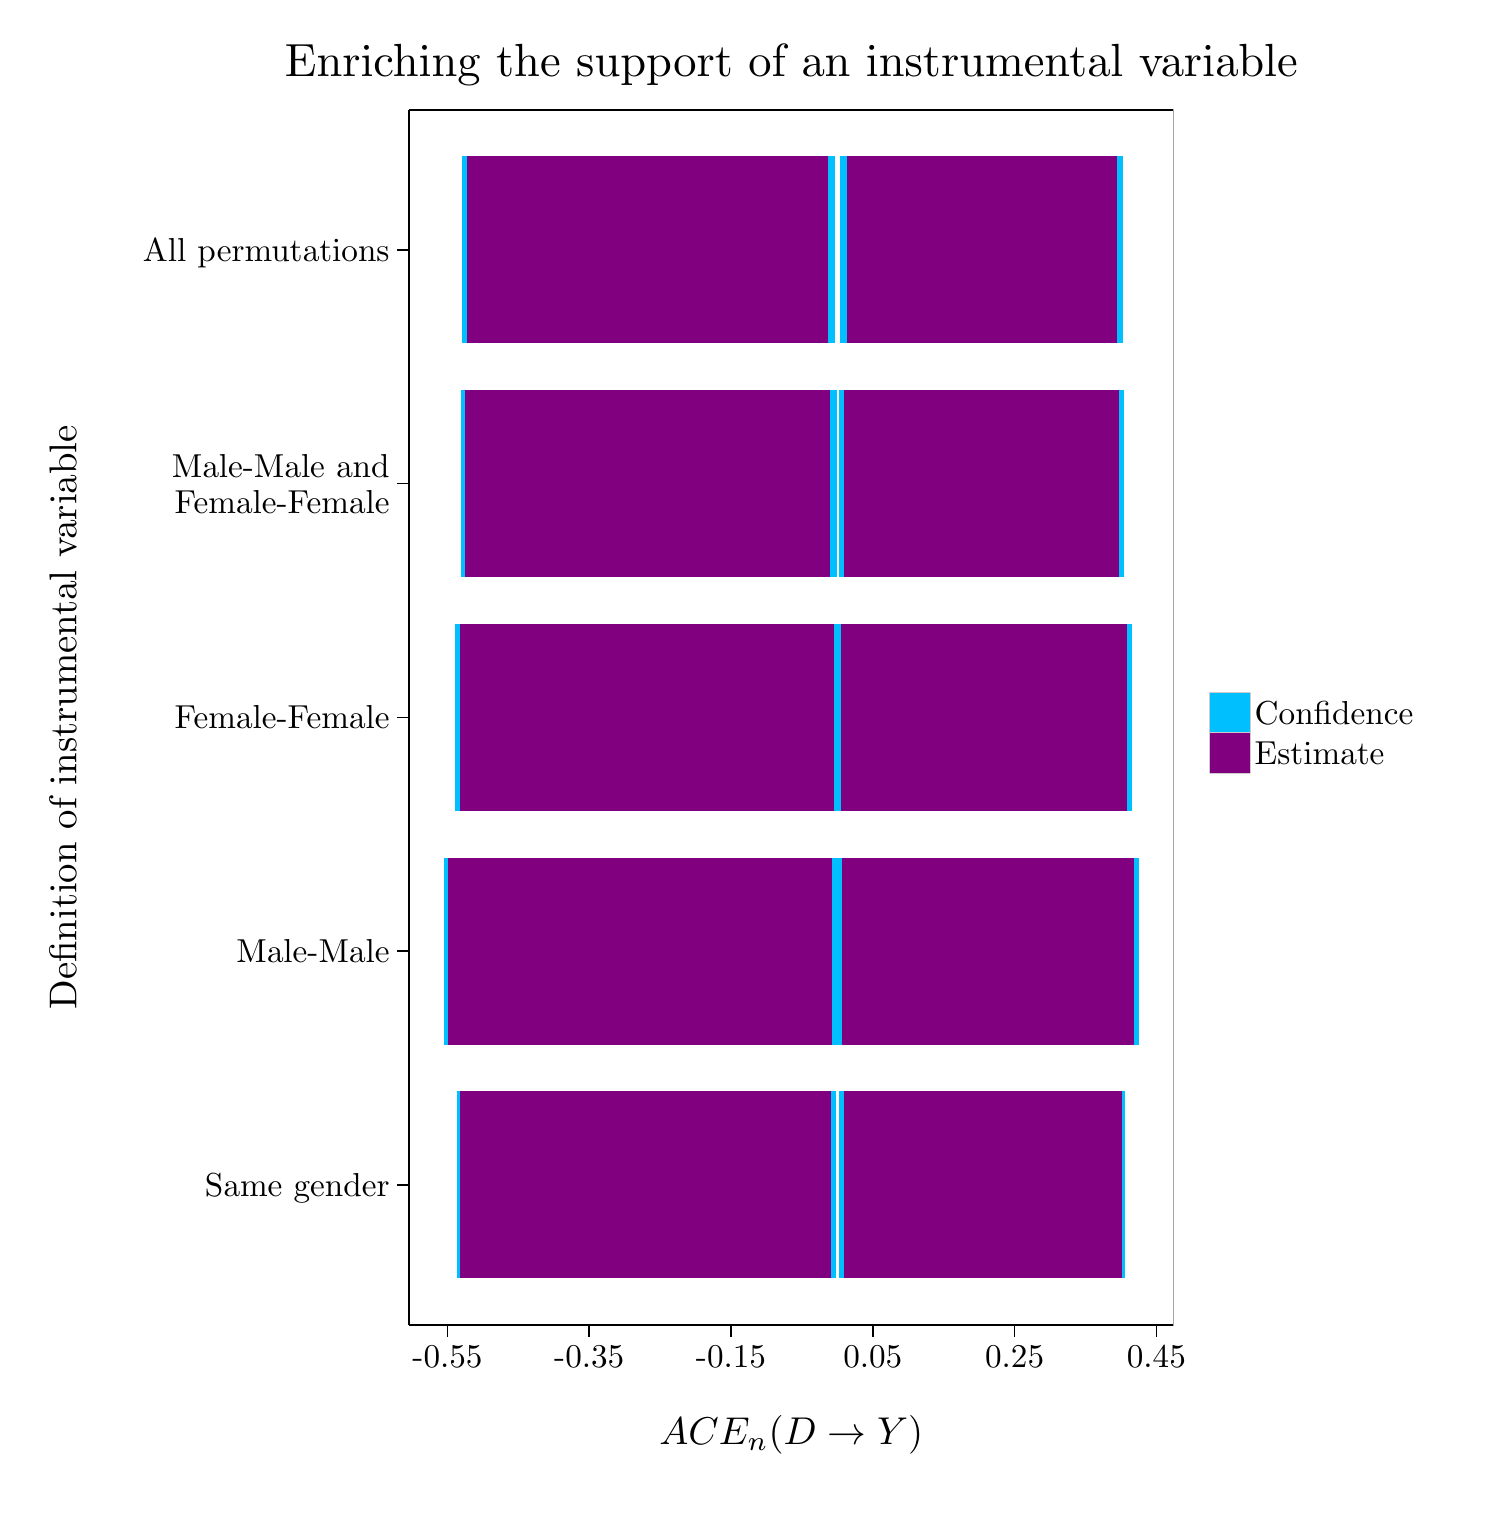
\begin{tikzpicture}[x=1pt,y=1pt]
\definecolor[named]{fillColor}{rgb}{1.00,1.00,1.00}
\path[use as bounding box,fill=fillColor,fill opacity=0.00] (-20,-25) rectangle (505.89,505.89);
\begin{scope}
\path[clip] (117.88, 37.06) rectangle (393.99,476.25);
\definecolor[named]{fillColor}{rgb}{0.00,0.75,1.00}

\path[fill=fillColor] (135.04, 53.96) rectangle (272.07,121.52);

\path[fill=fillColor] (130.43,138.42) rectangle (272.84,205.98);

\path[fill=fillColor] (134.53,222.87) rectangle (273.35,290.44);

\path[fill=fillColor] (136.58,307.33) rectangle (272.33,374.90);

\path[fill=fillColor] (136.83,391.79) rectangle (271.82,459.36);

\path[fill=fillColor] (273.10, 53.96) rectangle (376.58,121.52);

\path[fill=fillColor] (272.33,138.42) rectangle (381.44,205.98);

\path[fill=fillColor] (271.82,222.87) rectangle (378.88,290.44);

\path[fill=fillColor] (273.10,307.33) rectangle (376.06,374.90);

\path[fill=fillColor] (273.35,391.79) rectangle (375.81,459.36);
\definecolor[named]{fillColor}{rgb}{0.50,0.00,0.50}

\path[fill=fillColor] (136.32, 53.96) rectangle (270.28,121.52);

\path[fill=fillColor] (131.97,138.42) rectangle (270.79,205.98);

\path[fill=fillColor] (136.06,222.87) rectangle (271.30,290.44);

\path[fill=fillColor] (138.11,307.33) rectangle (270.02,374.90);

\path[fill=fillColor] (138.63,391.79) rectangle (269.26,459.36);

\path[fill=fillColor] (274.89, 53.96) rectangle (375.30,121.52);

\path[fill=fillColor] (274.38,138.42) rectangle (379.91,205.98);

\path[fill=fillColor] (273.87,222.87) rectangle (377.34,290.44);

\path[fill=fillColor] (275.15,307.33) rectangle (374.27,374.90);

\path[fill=fillColor] (275.91,391.79) rectangle (373.76,459.36);
\definecolor[named]{drawColor}{rgb}{0.00,0.00,0.00}

\path[draw=drawColor,line width= 0.6pt,line join=round,line cap=round] (117.88, 37.06) rectangle (393.99,476.25);
\end{scope}
\begin{scope}
\path[clip] (-20,-25) rectangle (505.89,505.89);
\definecolor[named]{drawColor}{rgb}{0.00,0.00,0.00}

\path[draw=drawColor,line width= 0.6pt,line join=round] (117.88, 37.06) --
	(117.88,476.25);
\end{scope}
\begin{scope}
\path[clip] (-20,-25) rectangle (505.89,505.89);
\definecolor[named]{drawColor}{rgb}{0.00,0.00,0.00}

\node[text=drawColor,anchor=base east,inner sep=0pt, outer sep=0pt, scale=  1.20] at (110.77, 83.61) {Same gender};

\node[text=drawColor,anchor=base east,inner sep=0pt, outer sep=0pt, scale=  1.20] at (110.77,168.07) {Male-Male};

\node[text=drawColor,anchor=base east,inner sep=0pt, outer sep=0pt, scale=  1.20] at (110.77,252.53) {Female-Female};

\node[text=drawColor,anchor=base east,inner sep=0pt, outer sep=0pt, scale=  1.20] at (110.77,343.47) {Male-Male and };

\node[text=drawColor,anchor=base east,inner sep=0pt, outer sep=0pt, scale=  1.20] at (110.77,330.51) { Female-Female};

\node[text=drawColor,anchor=base east,inner sep=0pt, outer sep=0pt, scale=  1.20] at (110.77,421.44) {All permutations};
\end{scope}
\begin{scope}
\path[clip] (-20,-25) rectangle (505.89,505.89);
\definecolor[named]{drawColor}{rgb}{0.00,0.00,0.00}

\path[draw=drawColor,line width= 0.6pt,line join=round] (113.61, 87.74) --
	(117.88, 87.74);

\path[draw=drawColor,line width= 0.6pt,line join=round] (113.61,172.20) --
	(117.88,172.20);

\path[draw=drawColor,line width= 0.6pt,line join=round] (113.61,256.66) --
	(117.88,256.66);

\path[draw=drawColor,line width= 0.6pt,line join=round] (113.61,341.12) --
	(117.88,341.12);

\path[draw=drawColor,line width= 0.6pt,line join=round] (113.61,425.58) --
	(117.88,425.58);
\end{scope}
\begin{scope}
\path[clip] (-20,-25) rectangle (505.89,505.89);
\definecolor[named]{drawColor}{rgb}{0.00,0.00,0.00}

\path[draw=drawColor,line width= 0.6pt,line join=round] (117.88, 37.06) --
	(393.99, 37.06);
\end{scope}
\begin{scope}
\path[clip] (-20,-25) rectangle (505.89,505.89);
\definecolor[named]{drawColor}{rgb}{0.00,0.00,0.00}

\path[draw=drawColor,line width= 0.6pt,line join=round] (131.71, 32.80) --
	(131.71, 37.06);

\path[draw=drawColor,line width= 0.6pt,line join=round] (182.94, 32.80) --
	(182.94, 37.06);

\path[draw=drawColor,line width= 0.6pt,line join=round] (234.16, 32.80) --
	(234.16, 37.06);

\path[draw=drawColor,line width= 0.6pt,line join=round] (285.39, 32.80) --
	(285.39, 37.06);

\path[draw=drawColor,line width= 0.6pt,line join=round] (336.62, 32.80) --
	(336.62, 37.06);

\path[draw=drawColor,line width= 0.6pt,line join=round] (387.85, 32.80) --
	(387.85, 37.06);
\end{scope}
\begin{scope}
\path[clip] (-20,-25) rectangle (505.89,505.89);
\definecolor[named]{drawColor}{rgb}{0.00,0.00,0.00}

\node[text=drawColor,anchor=base,inner sep=0pt, outer sep=0pt, scale=  1.20] at (131.71, 21.69) {-0.55};

\node[text=drawColor,anchor=base,inner sep=0pt, outer sep=0pt, scale=  1.20] at (182.94, 21.69) {-0.35};

\node[text=drawColor,anchor=base,inner sep=0pt, outer sep=0pt, scale=  1.20] at (234.16, 21.69) {-0.15};

\node[text=drawColor,anchor=base,inner sep=0pt, outer sep=0pt, scale=  1.20] at (285.39, 21.69) {0.05};

\node[text=drawColor,anchor=base,inner sep=0pt, outer sep=0pt, scale=  1.20] at (336.62, 21.69) {0.25};

\node[text=drawColor,anchor=base,inner sep=0pt, outer sep=0pt, scale=  1.20] at (387.85, 21.69) {0.45};
\end{scope}
\begin{scope}
\path[clip] (-20,-25) rectangle (505.89,505.89);
\definecolor[named]{drawColor}{rgb}{0.00,0.00,0.00}

\node[text=drawColor,anchor=base,inner sep=0pt, outer sep=0pt, scale=  1.40] at (255.94, -6.02) {$ACE_n(D\rightarrow Y)$};
\end{scope}
\begin{scope}
\path[clip] (-20,-25) rectangle (505.89,505.89);
\definecolor[named]{drawColor}{rgb}{0.00,0.00,0.00}

\node[text=drawColor,rotate= 90.00,anchor=base,inner sep=0pt, outer sep=0pt, scale=  1.40] at ( -2.40,256.66) {Definition of instrumental variable};
\end{scope}
\begin{scope}
\path[clip] (-20,-25) rectangle (505.89,505.89);
\definecolor[named]{fillColor}{rgb}{1.00,1.00,1.00}

\path[fill=fillColor] (402.86,232.27) rectangle (484.98,281.05);
\end{scope}
\begin{scope}
\path[clip] (-20,-25) rectangle (505.89,505.89);
\definecolor[named]{drawColor}{rgb}{0.80,0.80,0.80}
\definecolor[named]{fillColor}{rgb}{1.00,1.00,1.00}

\path[draw=drawColor,line width= 0.6pt,line join=round,line cap=round,fill=fillColor] (407.13,250.99) rectangle (421.58,265.44);
\end{scope}
\begin{scope}
\path[clip] (-20,-25) rectangle (505.89,505.89);
\definecolor[named]{fillColor}{rgb}{0.00,0.75,1.00}

\path[fill=fillColor] (407.13,250.99) rectangle (421.58,265.44);

\path[] (407.13,250.99) --
	(421.58,265.44);
\end{scope}
\begin{scope}
\path[clip] (-20,-25) rectangle (505.89,505.89);
\definecolor[named]{fillColor}{rgb}{0.00,0.75,1.00}

\path[fill=fillColor] (407.13,250.99) rectangle (421.58,265.44);

\path[] (407.13,250.99) --
	(421.58,265.44);
\end{scope}
\begin{scope}
\path[clip] (-20,-25) rectangle (505.89,505.89);
\definecolor[named]{drawColor}{rgb}{0.80,0.80,0.80}
\definecolor[named]{fillColor}{rgb}{1.00,1.00,1.00}

\path[draw=drawColor,line width= 0.6pt,line join=round,line cap=round,fill=fillColor] (407.13,236.53) rectangle (421.58,250.99);
\end{scope}
\begin{scope}
\path[clip] (-20,-25) rectangle (505.89,505.89);
\definecolor[named]{fillColor}{rgb}{0.50,0.00,0.50}

\path[fill=fillColor] (407.13,236.53) rectangle (421.58,250.99);

\path[] (407.13,236.53) --
	(421.58,250.99);
\end{scope}
\begin{scope}
\path[clip] (-20,-25) rectangle (505.89,505.89);
\definecolor[named]{fillColor}{rgb}{0.50,0.00,0.50}

\path[fill=fillColor] (407.13,236.53) rectangle (421.58,250.99);

\path[] (407.13,236.53) --
	(421.58,250.99);
\end{scope}
\begin{scope}
\path[clip] (-20,-25) rectangle (505.89,505.89);
\definecolor[named]{drawColor}{rgb}{0.00,0.00,0.00}

\node[text=drawColor,anchor=base west,inner sep=0pt, outer sep=0pt, scale=  1.20] at (423.39,254.08) {Confidence};
\end{scope}
\begin{scope}
\path[clip] (-20,-25) rectangle (505.89,505.89);
\definecolor[named]{drawColor}{rgb}{0.00,0.00,0.00}

\node[text=drawColor,anchor=base west,inner sep=0pt, outer sep=0pt, scale=  1.20] at (423.39,239.63) {Estimate};
\end{scope}
\begin{scope}
\path[clip] (-20,-25) rectangle (505.89,505.89);
\definecolor[named]{drawColor}{rgb}{0.00,0.00,0.00}

\node[text=drawColor,anchor=base,inner sep=0pt, outer sep=0pt, scale=  1.68] at (255.94,488.30) {Enriching the support of an instrumental variable};
\end{scope}
\end{tikzpicture}
